\documentclass[a4paper,11pt,dvipdfmx]{jsarticle}

\usepackage{bm}
\usepackage[dvipdfmx]{graphicx}
\usepackage[dvipdfmx]{color}
\usepackage{ascmac}
\usepackage{siunitx}
\usepackage{otf}
\pagestyle{plain}
\usepackage{float}
\usepackage[dvipdfmx]{hyperref}
\usepackage{pxjahyper}
\usepackage{here}
\usepackage{titlesec}
\titleformat*{\section}{\LARGE\bfseries}
\titleformat*{\subsection}{\normalsize\bfseries}
\usepackage{url}
\usepackage[table,xcdraw]{xcolor}
\hypersetup{% hyperrefオプションリスト
setpagesize=false,
 bookmarksnumbered=true,%
 bookmarksopen=true,%
 colorlinks=true,%
 linkcolor=blue,
 citecolor=blue,
}


\begin{document}
\newpage
\section{\LARGE{実験装置(担当:大谷)}}

\subsection{加速器}
今回の実験は、神戸大学深江キャンパスの敷地内にあるタンデム静電加速器を用いて行った。ペレットチェーンに電荷を乗せて高電圧ターミナルに運び上げ高電圧を発生させてイオンを加速する装置で、一つの高電圧で加速イオンの電荷を負から正へ変換して2回加速する装置を総称してタンデム加速器という。\cite{tandemu}タンデム加速器を用いて計測を行ったのは2020年1月4日$\sim$2020年1月11日である。今回の実験では最大エネルギー3MeVの陽子ビームを利用する。表\ref{aclgaiyou}に加速器の使用を、図\ref{aclphoto}に加速器の写真を、図\ref{aclkouzou}に加速器の構図を示す。

\begin{figure}[H]
    \centering
    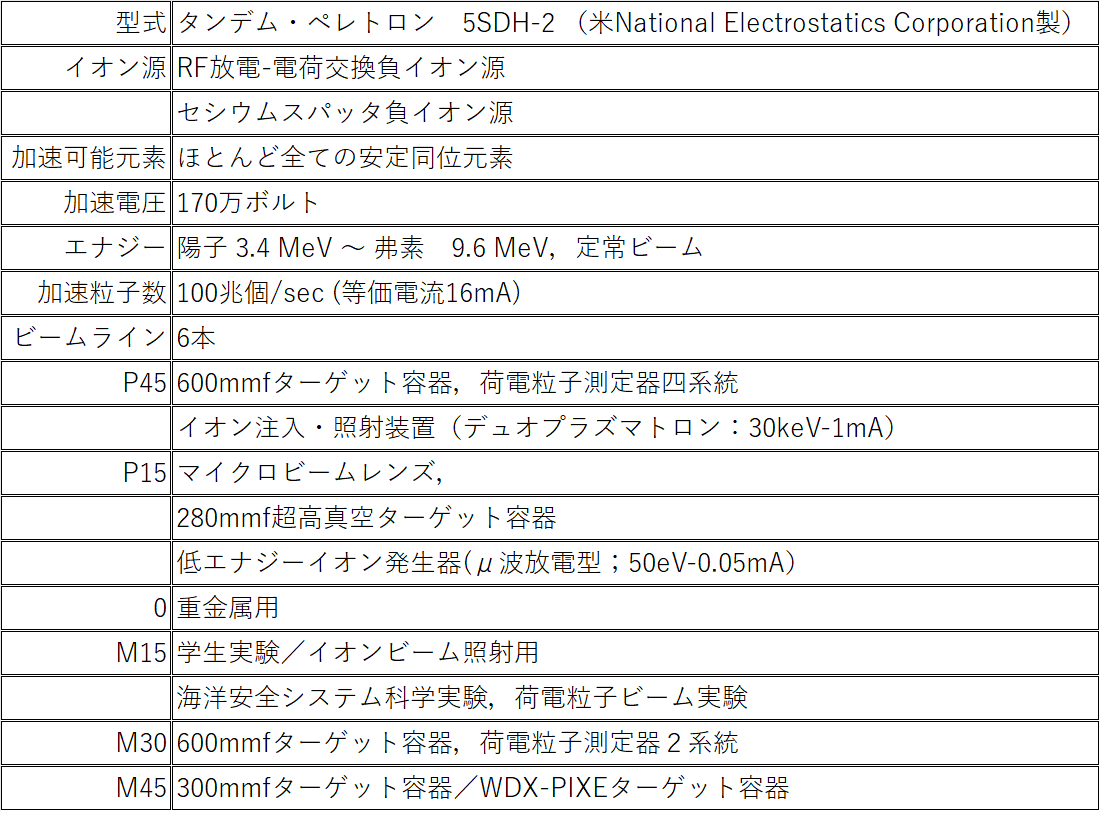
\includegraphics[width=90mm]{picture/setup/aclgaiyou.png}
    \caption{加速器の概要\cite{kasokukishiyou}}
    \label{aclgaiyou}
\end{figure}

\begin{figure}[H]
    \centering
    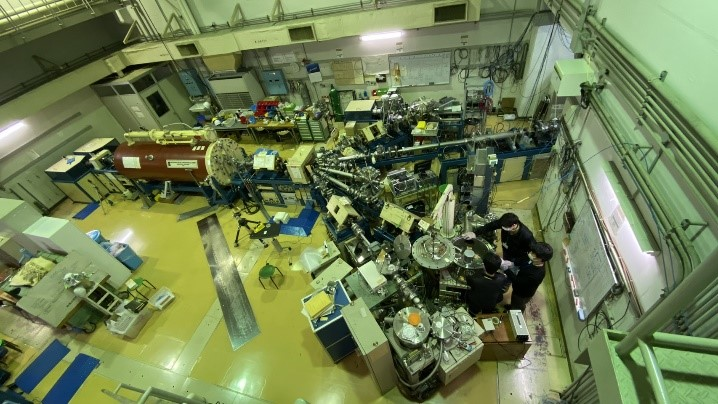
\includegraphics[width=90mm]{picture/setup/aclphoto.jpg}
    \caption{加速器の写真}
    \label{aclphoto}
\end{figure}

\begin{figure}[H]
    \centering
    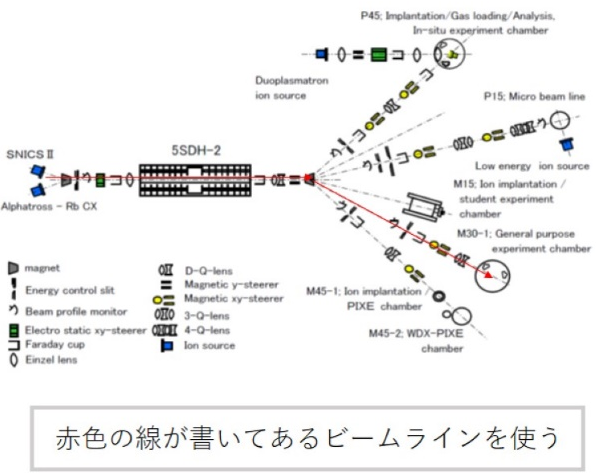
\includegraphics[width=80mm]{picture/setup/aclkouzou.png}
    \caption{加速器の構造\cite{beam}}
    \label{aclkouzou}
\end{figure}

\subsubsection{加速器本体}
加速器本体は、直径1.07m、長さ3.94mの円柱型である。負イオン源では原子に電子を結合させ負イオンを生成する。これを加速するため超高真空に保たれた初段加速管に入射し負イオン加速管入口まで到達させる。生成した負イオンは加速器タンクに入射し、タンク中央の正の電位を持った1.5MVの高電圧ターミナルと入射電極との電位差によって生成した電界によって加速される。このとき負イオンは1.5MeVに加速される。高電圧ターミナルに到達した負イオンは電子ストリッパー(窒素ガス層)で多数の電子がはぎ取られ正イオン(陽子)に変換される。生成した陽子は高電圧ターミナルと出口電極の間に生成した電界により再び加速される。ここで陽子はさらに1.5MeVに加速され、合計3MeVのエネルギーを持った陽子ビームとなる。加速されたビームは、二連四重極磁石によって収束された後、分析・振分電磁石により各ビームラインに偏光される。図\ref{aclmoshi}に加速器本体の模式図を示す。\cite{syousen}

\begin{figure}[H]
    \centering
    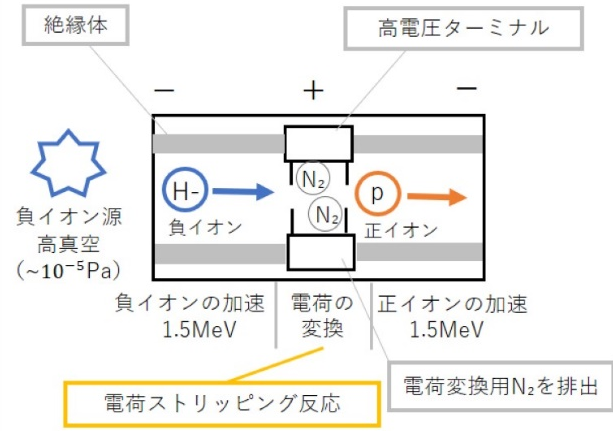
\includegraphics[width=70mm]{picture/setup/aclhonmoshi.png}
    \caption{加速器本体の模式図}
    \label{aclmoshi}
\end{figure}

\end{document}